% Copyright (C) 2014-2020 by Thomas Auzinger <thomas@auzinger.name>

\documentclass[draft,final]{vutinfth} % Remove option 'final' to obtain debug information.

% for displaying file structure
\usepackage{dirtree}
% Load packages to allow in- and output of non-ASCII characters.
\usepackage{lmodern}        % Use an extension of the original Computer Modern font to minimize the use of bitmapped letters.
\usepackage[T1]{fontenc}    % Determines font encoding of the output. Font packages have to be included before this line.
\usepackage[utf8]{inputenc} % Determines encoding of the input. All input files have to use UTF8 encoding.

% Extended LaTeX functionality is enables by including packages with \usepackage{...}.
\usepackage{amsmath}    % Extended typesetting of mathematical expression.
\usepackage{amssymb}    % Provides a multitude of mathematical symbols.
\usepackage{mathtools}  % Further extensions of mathematical typesetting.
\usepackage{microtype}  % Small-scale typographic enhancements.
\usepackage[inline]{enumitem} % User control over the layout of lists (itemize, enumerate, description).
\usepackage{multirow}   % Allows table elements to span several rows.
\usepackage{booktabs}   % Improves the typesettings of tables.
\usepackage{listings}   % Improves the typesettings of tables.
\usepackage{subcaption} % Allows the use of subfigures and enables their referencing.
\usepackage[ruled,linesnumbered,algochapter]{algorithm2e} % Enables the writing of pseudo code.
\usepackage[usenames,dvipsnames,table]{xcolor} % Allows the definition and use of colors. This package has to be included before tikz.
\usepackage{nag}       % Issues warnings when best practices in writing LaTeX documents are violated.
\usepackage{float} % Provides tooltip-like todo notes.
\usepackage{todonotes} % Provides tooltip-like todo notes.
\usepackage{hyperref}  % Enables cross linking in the electronic document version. This package has to be included second to last.
\usepackage{svg}
\usepackage[acronym,toc]{glossaries} % Enables the generation of glossaries and lists fo acronyms. This package has to be included last.
\usepackage{pdfpages}
% Define convenience functions to use the author name and the thesis title in the PDF document properties.
\newcommand{\authorname}{Dragana Sunaric} % The author name without titles.
\newcommand{\thesistitle}{How to Model and Transform Executable BPMN Process Models} % The title of the thesis. The English version should be used, if it exists.

% Set PDF document properties
\hypersetup{
    pdfpagelayout   = TwoPageRight,           % How the document is shown in PDF viewers (optional).
    linkbordercolor = {Melon},                % The color of the borders of boxes around crosslinks (optional).
    pdfauthor       = {\authorname},          % The author's name in the document properties (optional).
    pdftitle        = {\thesistitle},         % The document's title in the document properties (optional).
    pdfsubject      = {Subject},              % The document's subject in the document properties (optional).
    pdfkeywords     = {a, list, of, keywords} % The document's keywords in the document properties (optional).
}



\usepackage{bera}% optional: just to have a nice mono-spaced font
\definecolor{maroon}{rgb}{0.5,0,0}
\definecolor{darkgreen}{rgb}{0,0.5,0}
\colorlet{punct}{red!60!black}
\definecolor{background}{HTML}{EEEEEE}
\definecolor{delim}{RGB}{20,105,176}
\colorlet{numb}{magenta!60!black}


\definecolor{MyLightGray}{RGB}{252,252,252}
\definecolor{MyBlue}{RGB}{5,102,141}
\definecolor{MyGreen}{RGB}{0,168,150}
\definecolor{MyBrown}{RGB}{143,89,3}
\definecolor{MyOrange}{RGB}{213,111,30}

\lstdefinelanguage{json}{
	% Code styles
	keywords={effectedElements,id,name, type,title,description,details},
	basicstyle=\ttfamily\small,
	% texcsstyle=*\color{MyOrange},			% Tex control sequences
	% directivestyle=\color{MyOrange},		% Directives
	identifierstyle=\color{MyBlue},			% Identifiers
	commentstyle=\color{MyBrown}\itshape,   % Comments
	keywordstyle=\color{MyOrange}\bfseries,	% Keywords
	stringstyle=\color{MyGreen},     		% String literals
	numbers=left,
	numberstyle=\scriptsize,
	stepnumber=1,
	numbersep=8pt,
	showstringspaces=false,
	breaklines=true,
	literate=
	*{0}{{{\color{numb}0}}}{1}
	{1}{{{\color{numb}1}}}{1}
	{2}{{{\color{numb}2}}}{1}
	{3}{{{\color{numb}3}}}{1}
	{4}{{{\color{numb}4}}}{1}
	{5}{{{\color{numb}5}}}{1}
	{6}{{{\color{numb}6}}}{1}
	{7}{{{\color{numb}7}}}{1}
	{8}{{{\color{numb}8}}}{1}
	{9}{{{\color{numb}9}}}{1}
	{:}{{{\color{MyBrown}{:}}}}{1}
	{,}{{{\color{MyBrown}{,}}}}{1}
	{\{}{{{\color{MyBrown}{\{}}}}{1}
	{\}}{{{\color{MyBrown}{\}}}}}{1}
	{[}{{{\color{MyBrown}{[}}}}{1}
	{]}{{{\color{MyBrown}{]}}}}{1},
}
\lstdefinelanguage{xml}
{
	% Code styles
	basicstyle=\ttfamily\small,
	% texcsstyle=*\color{MyOrange},			% Tex control sequences
	% directivestyle=\color{MyOrange},		% Directives
	identifierstyle=\color{black},			% Identifiers
	commentstyle=\color{MyBrown}\itshape,   % Comments
	keywordstyle=\color{MyBlue}\bfseries,	% Keywords
	stringstyle=\color{MyGreen},    
	numbers=left,
	numberstyle=\scriptsize,
	stepnumber=1,
	numbersep=8pt,
	showstringspaces=false,
	breaklines=true,
	morestring=[s]{"}{"},
	morecomment=[s]{?}{?},
	morecomment=[s]{!--}{--},
	commentstyle=\color{MyGreen},
	moredelim=[s][\color{black}]{>}{<},
	moredelim=[s][\color{MyBrown}]{\ }{=},
	stringstyle=\color{MyBlue},
	identifierstyle=\color{MyOrange}
}

\setpnumwidth{2.5em}        % Avoid overfull hboxes in the table of contents (see memoir manual).
\setsecnumdepth{subsection} % Enumerate subsections.

\nonzeroparskip             % Create space between paragraphs (optional).
\setlength{\parindent}{0pt} % Remove paragraph identation (optional).

\makeindex      % Use an optional index.
\makeglossaries % Use an optional glossary.
%\glstocfalse   % Remove the glossaries from the table of contents.

% Set persons with 4 arguments:
%  {title before name}{name}{title after name}{gender}
%  where both titles are optional (i.e. can be given as empty brackets {}).
\setauthor{}{\authorname}{}{female}
\setadvisor{Ao.Univ.Prof. Dipl.-Inf. Dr.-Ing.}{Jürgen Dorn}{}{male}

% For bachelor and master theses:
%\setfirstassistant{Pretitle}{Forename Surname}{Posttitle}{male}
%\setsecondassistant{Pretitle}{Forename Surname}{Posttitle}{male}
%\setthirdassistant{Pretitle}{Forename Surname}{Posttitle}{male}

% Required data.
\setregnumber{11814569}
\setdate{01}{01}{2022} % Set date with 3 arguments: {day}{month}{year}.
\settitle{\thesistitle}{Vereinfachung von BPMN-Diagrammen} % Sets English and German version of the title (both can be English or German). If your title contains commas, enclose it with additional curvy brackets (i.e., {{your title}}) or define it as a macro as done with \thesistitle.
%\setsubtitle{Optional Subtitle of the Thesis}{Optionaler Untertitel der Arbeit} % Sets English and German version of the subtitle (both can be English or German).

% Select the thesis type: bachelor / master / doctor / phd-school.
% Bachelor:
\setthesis{bachelor}
%
% Master:
%\setthesis{master}
%\setmasterdegree{dipl.} % dipl. / rer.nat. / rer.soc.oec. / master
%
% Doctor:
%\setthesis{doctor}
%\setdoctordegree{rer.soc.oec.}% rer.nat. / techn. / rer.soc.oec.
%
% Doctor at the PhD School
%\setthesis{phd-school} % Deactivate non-English title pages (see below)

% For bachelor and master:
\setcurriculum{Software \& Information Engineering}{Software \& Information Engineering} % Sets the English and German name of the curriculum.

% For dissertations at the PhD School:
\setfirstreviewerdata{Affiliation, Country}
\setsecondreviewerdata{Affiliation, Country}


\begin{document}

% adding glossarys 
\newacronym{bpm}{BPM}{Business Process Management}
\newacronym{bpmn}{BPMN}{Business Process Model and Notation}
\newacronym{bpms}{BPMS}{\gls{bpmn-engine}}
\newacronym{XML}{XML}{Extensible Markup Language \gls{xml}}
\newacronym{XSD}{XSD}{XML Schema Definition \gls{xsd}}
\newglossaryentry{bpmn-wokflow-management-system}
{
	name={BPMN Workflow Management System},
	description={A software for executing workflows specified as \gls{bpmn} models}
}
\newglossaryentry{bpmn-engine}
{
	name={Business Process Workflow Management System},
	description={see \gls{bpmn-wokflow-management-system}}
}

\newglossaryentry{executable-bpmn}
{
	name={executable \gls{bpmn} model},
	description={A software for executing workflows specified as \gls{bpmn} models}
}

\newglossaryentry{happy-path}
{
	name={'happy-path'},
	description={The best-case scenario in a process}
}

\newglossaryentry{conceptual-bpmn}
{
	name={conceptual \gls{bpmn} model},
	description={A \gls{bpmn} model describing a business process that cannot be directly executed on a \gls{bpmn-engine}}
}

\newglossaryentry{business-oriented-bpmn}
{
	name={business-oriented process model},
	description={See \gls{conceptual-bpmn}}
}
\newglossaryentry{automated-task}
{
	name={Automated task},
	description={A task that can be automated in a \gls{bpmn-wokflow-management-system}}
}

\newglossaryentry{service-task}
{
	name={Service Task},
	description={``Task that uses some sort of service, which could be a Web service or an automated application``\cite[p.~158]{bpmnstandard} }
}
\newglossaryentry{send-task}
{
	name={Send Task},
	description={``designed to send a Message to an external Participant``[p.~159]\cite{bpmnstandard} }
}
\newglossaryentry{receive-task}
{
	name={Receive Task},
	description={``designed to wait for a Message to arrive from an external Participant``[p.~161]\cite{bpmnstandard} }
}
\newglossaryentry{businessrule-task}
{
	name={Business Rule Task},
	description={``provides a mechanism for the Process to provide input to a Business Rules Engine and to get the output of calculations that the Business Rules Engine might provide``[p.~163]\cite{bpmnstandard} }
}
\newglossaryentry{script-task}
{
	name={Script Task},
	description={``executed by a business process engine. The modeler or implementer defines a script in a language that the engine can interpret``[p.~164]\cite{bpmnstandard} }
}
\newglossaryentry{manual-task}
{
	name={Manual Task},
	description={``A Task that is expected to be performed without the aid of any business process execution engine``[p.~163]\cite{bpmnstandard} }
}
\newglossaryentry{user-task}
{
	name={User Task},
	description={``A typical “workflow” Task where a human performer performs the Task with the assistance of a software application``[p.~163]\cite{bpmnstandard} }
}
\newglossaryentry{data-store}
{
	name={Data Store},
	description={``A DataStore provides a mechanism for Activities to retrieve or update stored information that will persist beyond the
		scope of the Process``[p.~208]\cite{bpmnstandard} }
}

\newglossaryentry{data-object}
{
	name={Data Object},
	description={``Data Objects representing a Collection of Data``[p.~206]\cite{bpmnstandard} }
}
\newglossaryentry{xml}
{
	name={XML},
	description={Extensible Markup Language - Defined by W3C\cite{bray1997extensibl} }
}

\newglossaryentry{xsd}
{
	name={XSD},
	description={XML Schema Definition - Definition of the stucture of a XML File\cite{bray1997extensibl} }
}

\frontmatter % Switches to roman numbering.
% The structure of the thesis has to conform to the guidelines at
%  https://informatics.tuwien.ac.at/study-services

%\addtitlepage{naustrian} % German title page (not for dissertations at the PhD School).

\selectlanguage{english}
\addtitlepage{english} % English title page.

\AddStatementPage



\begin{acknowledgements*}
	\todo{write Acknowledgements}

\end{acknowledgements*} % A short introduction to LaTeX.

\begin{abstract}	
BPMN is a commonly used diagramming language to visualize business processes. Executable process models are an effective tool for bridging the gap between IT experts, that are responsible for process automation, and domain experts, who have insight knowledge about the process at hand. This thesis explains best practices for modeling efficient executable BPMN process models and gives suggestions on how executable process models can be transformed to improve expressiveness and readability.  

Some of those best practices and suggestions can be automated, therefore a software was implemented as part of this thesis that can scan a BPMN model for violations of mentioned best practices. This software is freely available as an open source project on github:  \url{https://github.com/dsunaric/epms-service}. 

This thesis goes then on to demonstrate in a case study how the software can be used as an aid to implement the suggestions. The process used for this case study originated from a real live client registration process used in the telecommunication sector and was adapted to be used in this thesis.

In practice there may be cases where some of the suggestions mentioned in this thesis will not be suited (e.g. when activities have to be kept for legal reasons).
\end{abstract}

% Select the language of the thesis, e.g., english or naustrian.

% Add a table of contents (toc).
\tableofcontents % Starred version, i.e., \tableofcontents*, removes the self-entry.

% Switch to arabic numbering and start the enumeration of chapters in the table of content.
\mainmatter

\chapter{Introduction}
\gls{bpmn} is an widely used and established diagramming language with the purpose of visualizing business processes in organizations. Process models are usually created by process analysts together with domain experts. \gls{bpmn}-models created that way contain incomplete and implicit information for the specific business domain and are therefore called \gls{conceptual-bpmn}. By involving IT-experts these \gls{conceptual-bpmn}s can be made executable and automated using a \gls{wfms}. \cite{fundamentals}

Today \gls{wfms}s like \gls{camunda}  and \gls{alfresco} are widely used by big organizations \cite{camunda-customers} \cite{activity-customers}. Real-life processes being executed in \gls{wfms}s can be complex and have to be changed and reevaluated together with the software embedded in these processes as requirements and guidelines for the specific domain change. 

One advantage of directly automating processes defined as \gls{bpmn} is its readability for IT-experts and domain-experts. As a consequence both parties have a common understanding of the process that is executed and have basis for discussion when changes have to be made. In order for the cooperation between IT and business to work smoothly, \gls{executable-bpmn} should be as simple to understand as possible and be in line with known standards and best practices. 

Applying guidelines for good \gls{executable-bpmn}s does not only increase readability but can also have direct impact on process costs. Due to the pricing scheme of some enterprise \gls{wfms}s, which take into account the total number of nodes passed by process instances, eliminating non necessary handovers and therefore reducing the number of nodes in the \gls{bpmn} model, can have an impact on the required license. 

\section{Goal of This Thesis}
The goal of this thesis is to give practical guidance on how to apply best practices and methodologies to create good \gls{executable-bpmn}s and to improve existing models. 

This will be achieved by stating the current research on creating \gls{executable-bpmn}s. After that this work will take a look at methods for transforming and improving existing \gls{executable-bpmn}s and how to use them to create models in line with the stated best practices. In order to compare two process models, this work will also provide methods for measuring metrics like time and cost of processes defined as \gls{bpmn} models. Finally this thesis will provide detailed information about how to use these methods in practice with a case study.

\section{Structure of This Thesis}
This Thesis starts with an state-of-the-art section consisting of two chapters. The first one is about the nature of \gls{executable-bpmn}s and how to make an existing \gls{conceptual-bpmn} executable by an \gls{wfms}. The second chapter provides methods for analyzing and improving processes using Six Sigma approaches and quantifiable measures.

Along with this thesis a software was developed which suggest changes to an \gls{executable-bpmn} given as an \gls{XML}-file based on the best practices found in the first two chapters. The documentation and implementation details on this software can be found in chapter 4. 

Not every aspect of transformation given in the first two chapters is suitable to be fully automated and requires knowledge on the specific domain of the process. Therefore, the last chapter provides a case-study to an existing process model applying the principles from the first two chapters and giving a guide on how to use those principles in practice.

\chapter{Automating Business Processes}
\label{chapter-2}
The following chapter will provide an overview of the current research on best practices when creating executable \gls{bpmn} models. First, it will discuss the motivation behind process automation and using \gls{wfms}s and the benefit it might bring to an organization. Then it will state the differences between an \gls{conceptual-bpmn}, that cannot be deployed on an \gls{wfms}, and an \gls{executable-bpmn}. Finally, this chapter will list the steps necessary to turn an \gls{conceptual-bpmn} executable.

\section{Why Automate Processes?}
Introducing an \gls{wfms} in an organization is often done to open the possibilities of automating parts of a process or even the whole process. While process automation in itself can be useful, there are some other advantages of introducing an \gls{wfms}, besides the possibility to automate certain process steps.

\subsection{Shorten Process Lifetime}
Managing processes manually requires handling tasks such as handling handovers from one entity to another. This can lead to unnecessary waiting periods between two tasks. By implementing an \gls{wfms} resource allocation and parallelization can be automated where possible to assure optimal use of process resources. \cite{gadatsch2020grundkurs}

\subsection{Reduce Process Cost}
By reducing process lifetimes and increasing productivity due to better handling of resources process costs can be reduced \cite{gadatsch2020grundkurs}. in this context, it has to be said, that due to the high price for workflow management systems the overall cost does not have to decrease necessarily after implementing an \gls{wfms} \cite{gruber2009profitability}.

\subsection{Workload Reduction}
As stated earlier, managing processes needs to be done either by an \gls{wfms} or manually which creates an additional workload for an organization. Workloads for employees executing the processes are also kept steady due to dynamic resource assignments. \cite{fundamentals}\cite{gadatsch2020grundkurs}

\subsection{Enforce Rules}
Defining the processes that are directly executed and controlled by an \gls{wfms} enables the organization to enforce the execution of the process as it is designed without giving employees room for shortcuts. Following rules and protocols regarding the process can be automated and enforcing guidelines and laws in an organization becomes easier. \cite{fundamentals}

\subsection{Create Transparency}
Using an \gls{wfms} provides insights into the actual processes that are executed in the organization. This makes it easier to determine the performance of processes by providing historical information of completed process instances and provides insight into the current status of processes that are still in progress. \cite{gadatsch2020grundkurs}

\section{Executable vs Conceptual Process Models}
Process models are inherently business-oriented as their purpose is initially to define and visualize the processes happening in an organization. Business-oriented or \gls{conceptual-bpmn} are meant to be read by domain experts and contain usually implicit information known to these experts \cite{fundamentals}. They are typically incomplete, meaning that not every possible outcome of a process is modeled. In fact, usually only the best-case scenario, also known as the \gls{happy-path}, of a process is modeled in an \gls{conceptual-bpmn} \cite{freund2019real}.\\~\\Due to their incompleteness, business-oriented models cannot be executed in an \gls{wfms} just like that but have to be turned into an \gls{executable-bpmn}. \gls{executable-bpmn} are meant for IT experts and should be a technical representation of the business process while still begin readable by domain experts. They should leave no room for interpretation as they have to contain all the information necessary for the process to be executed by an \gls{wfms}. Besides the visual information, \gls{executable-bpmn} also need to contain execution properties like interface definitions and variables that are used by the process. Those variables are called \gls{process-variables}.\cite{fundamentals} \\~\\An algorithm on how to efficiently turn an \gls{conceptual-bpmn} executable as stated in the book \textit{Fundamentals of Business Process Management} \cite{fundamentals} is described in the next section. 

\section{Making Process Models Executable}
As stated earlier, \gls{bpmn} models can not directly be executed by a \gls{bpms} but have to be converted from an \gls{conceptual-bpmn} into an \gls{executable-bpmn}. 

There are different approaches to how this conversion can take place. In \cite{fundamentals} performing such a transformation is broken down into 5 steps:
\begin{enumerate}
	\item Identify the automation boundaries
	\item Review manual tasks
	\item Complete the process model
	\item Bring the process model to an adequate granularity level
	\item Specify execution properties
\end{enumerate}

\subsection{Identify the Automation Boundaries}\label{automation}
The first step in turning an \gls{conceptual-bpmn} in an  \gls{executable-bpmn} is to identify which steps can be automated using a \gls{wfms}. 

Tasks which can inherently be automated are called \gls{automated-task}s \cite[p.~317]{fundamentals}. Taking a look at the BPMN 2.0 standard an \gls{automated-task} can be one of the following Task types:
\begin{itemize}
	\item \textbf{\gls{service-task}}: A Task that invokes a service. This service can be a webservice or application code.
	\item \textbf{\gls{send-task}}: Used to send a message to an external participant (A participant that is not part of the process).
	\item \textbf{\gls{receive-task}}: Used to receive a message from an external participant. 
	\item \textbf{\gls{script-task}}: Executes a script that can be interpreted by the \gls{wfms}.
	\item \textbf{\gls{businessrule-task}}: Executes a rule. (e.g. provides input for a business rule engine and gets the output of that calculation)
\end{itemize}

\begin{figure}[H]
	\centering
	\begin{subfigure}[b]{0.18\columnwidth}
		\centering
		\includegraphics[width=0.9\textwidth]{graphics/service-task}
		\subcaption{Service Task}
		\label{fig:servicetask}
	\end{subfigure}
	\begin{subfigure}[b]{0.18\columnwidth}
		\centering
		\includegraphics[width=0.9\columnwidth]{graphics/send-task}
		\subcaption{Send Task}
		\label{fig:sendtask}
	\end{subfigure}
	\begin{subfigure}[b]{0.18\columnwidth}
		\centering
		\includegraphics[width=0.9\columnwidth]{graphics/receive-task}
		\subcaption{Receive Task}
		\label{fig:receivetask}
	\end{subfigure}
	\begin{subfigure}[b]{0.18\columnwidth}
		\centering
		\includegraphics[width=0.9\columnwidth]{graphics/script-task}
		\subcaption{Script Task}
		\label{fig:scripttask}
	\end{subfigure}
	\begin{subfigure}[b]{0.24\columnwidth}
		\includegraphics[width=0.675\columnwidth]{graphics/businessrule-task}
		\subcaption{Business rule Task}
		\label{fig:businessruletask}
	\end{subfigure}
	\caption{Automated tasks according to the BPMN 2.0 standard \cite{bpmnstandard}} % Remove the [...] argument if the original caption should be used in the figure list.
	\label{fig:automatedtasks} % \label has to be placed AFTER \caption (or \subcaption) to produce correct cross-references.
\end{figure}

Usually, not every step in a process can be fully automated. Processes can also have \textbf{manual tasks} and \textbf{user tasks}. While both describe activities performed by humans,\textbf{user tasks} are aided by the orchestration and resource management functionalities of a \gls{wfms} and \textbf{manual tasks} do not interact with the business process execution engine at all. 

\begin{figure}[h]
	\centering
	\begin{subfigure}[b]{0.18\columnwidth}
		\centering
		\includegraphics[width=0.9\textwidth]{graphics/user-task}
		\subcaption{User Task}
		\label{fig:usertask}
	\end{subfigure}
	\begin{subfigure}[b]{0.18\columnwidth}
		\centering
		\includegraphics[width=0.9\columnwidth]{graphics/manual-task}
		\subcaption{Manual Task}
		\label{fig:manualtask}
	\end{subfigure}
	\caption{Manual and user tasks according to the BPMN 2.0 standard \cite{bpmnstandard}} % Remove the [...] argument if the original caption should be used in the figure list.
	\label{fig:nonautomatedtasks} % \label has to be placed AFTER \caption (or \subcaption) to produce correct cross-references.
\end{figure}

\subsection{Review Manual Tasks}\label{manual}
As mentioned earlier manual tasks are not automated and do also happen without the aid of a \gls{wfms}. Most \gls{wfms} implement manual tasks as a pass-through activity, meaning the manual task is ignored \cite{manual-activity}\cite{manual-camunda}\cite{manual-bizagi}. To incorporate all aspects of the process into the \gls{wfms}, it is necessary to evaluate if the identified manual tasks in our \gls{bpmn}-model can be substituted by other BPMN constructs. This can be done in the following ways:
\begin{itemize}
	\item \textbf{Automate the task}: Trying to extend the current automation boundaries would be the best case scenario \gls{receive-task}. Depending on the nature of the task that is currently performed manually, this might not always be possible. 
	
	\item \textbf{Turn it into a user task}: If the task cannot be automated or the organization lacks the resources to automate the task yet, another possibility is to change the manual task into a user task. The \gls{wfms} manages task assignments and after completion, the system is notified via a worklist handler. \cite{stefanov2014business}
\end{itemize}

In the case that neither an automated task nor a user task is suitable for modeling the manual task, one might also consider isolating the task and modeling the rest of the process. If this is also not possible, due to the manual task being crucial for the expressiveness of the model, it might be reconsidered if this process can or should be considered to be executed using a \gls{wfms}\cite[p.~228]{freund2019real}

\subsection{Complete the Process Model}\label{complete}
Usually, \gls{conceptual-bpmn}s are not complete and leave out certain information that is seen as implicit knowledge or as not important by the person modeling the process. These gaps in the model might be crucial when a complete picture of the process is needed for automation. 

A common incompleteness in many conceptual models is ignoring errors and only implementing the \gls{happy-path} of a process. The \gls{happy-path} is the best-case scenario that can happen in the execution of a process. While it might be sufficient for a conceptual model, the corresponding executable BPMN model has to define what happens in case any error occurs. 

Apart from defining alternative process paths, in this step of turning a model executable, it is also necessary to model the input and output data of tasks and gateways. In the BPMN 2.0 specification this is done using \gls{data-store}s and \gls{data-object}s. 

\begin{figure}[H]
	\centering
	\begin{subfigure}[b]{0.18\columnwidth}
		\centering
		\includegraphics[width=0.9\columnwidth]{graphics/data-store}
		\caption{Data Store} 
		\label{fig:datastore} 
	\end{subfigure}
	\begin{subfigure}[b]{0.18\columnwidth}
		\centering
		\includegraphics[width=0.8\columnwidth]{graphics/data-object}
		\subcaption{Data Object}
		\label{fig:dataobject}
	\end{subfigure}
	\caption{Data store and data objects according to the BPMN 2.0 standard \cite{bpmnstandard}} % Remove the [...] argument if the original caption should be used in the figure list.
	\label{fig:datastoreandobject} % \label has to be placed AFTER \caption (or \subcaption) to produce correct cross-references.
\end{figure}

\subsection{Bring the Process Model to an Adequate Granularity Level}\label{granulartity}
The granularity of tasks in an \gls{conceptual-bpmn} does differ from the granularity needed in an \gls{executable-bpmn}.
As mentioned before, using an \gls{wfms} is not just about the possibility of automation, but mainly the orchestration and deciding who needs to be doing which task. \cite{freund2019real}
\\~\\Therefore consecutive tasks that are done by the same participant should be clustered together to minimize handovers that have to be unnecessarily processed by the workflow management system. \cite{fundamentals}
However, there are some exceptions to this rule:
\begin{itemize}
	\item \textbf{Tracking progress}: To know how much the process has advanced, it can be useful to split certain tasks even if they are done by the same participant. 
	\item \textbf{Handling exceptions}: If different errors and exceptions can occur for a set of tasks that is performed by the same participant, it is recommended to keep these tasks separated.
	\item \textbf{Managing resources}: Sometimes consecutive tasks are performed by participants that have the same role, but could be done by two different participants to maximize capacity. In this case, it is also recommended to dis-aggregate the task accordingly.
\end{itemize}

\subsection{Specify Execution Properties}
The final step in turning an \gls{conceptual-bpmn} executable is to specify the implementation details of our \gls{bpmn} model. While the changes performed up to this step had an impact of the graphical rendering, the execution properties are not graphically embedded into \gls{bpmn} but are encoded into the \gls{XML} specification of the BPMN-model. \cite{fundamentals} A schematic representation of the structure of \gls{bpmn} is provided in figure \ref{fig:bpmn-schema}. For an insight in the full specification of the BPMN 2.0 XML, the \gls{xml}-schema can be found on the OMG-Website\cite{BPMN-xml-spec}. 
\begin{figure}[H]
	\centering
	\includegraphics[width=0.3\columnwidth]{graphics/bpmn-schema}
	\caption{Structure of the BPMN format \cite{fundamentals}} 
	\label{fig:bpmn-schema} 
\end{figure}


\paragraph{Process Variables}~\\
To use data in different elements of our process, we need process variables that can be read, created, and modified during the process's execution. Every Process variable has a \textbf{data type} that can either be simple (strings, integers, doubles, booleans, dates, times, ...) or complex (composed of other types). A complex type needs to be described as an \gls{XSD}-schema file as shown in listing \ref{lst:schema-person}. 

\begin{lstlisting}[language=xml,caption={The \gls{xml}-Schema Definiton for a complex type 'person'},captionpos=b, label={lst:schema-person}]
	<xs:element name="person">
	<xs:complexType>
	<xs:sequence>
	<xs:element name="name" type="xs:string"/>
	<xs:element name="address" type="xs:string"/>
	<xs:element name="city" type="xs:string"/>
	<xs:element name="country" type="xs:string"/>
	</xs:sequence>
	</xs:complexType>
	</xs:element>
\end{lstlisting}

The corresponding complex XML object can be seen in listing \ref{lst:data-person}. 
\begin{lstlisting}[language=xml,caption={An instance of the complex type 'person'},captionpos=b,label={lst:data-person}]
	<person>
	<name>Dragana Sunaric</name>
	<address>Wiedner-Hauptstrasse 5</address>
	<city>1040 Wien</city>
	<country>Austria</country>
	</person>
\end{lstlisting}


~\\The definition of common errors, messages, and escalations that are either thrown or listened to by events and tasks are also part of the execution properties. 
\paragraph{Messages}~\\
Every BPMN element has at least an \textbf{id} that identifies the given element and a descriptive \textbf{name} of the element.\cite{bpmnstandard} Despite the properties that all BPMN elements have, messages have no additional variables that need to be set. An example of a message specification can be seen in listing \ref{lst:message}.
\begin{lstlisting}[language=xml,caption={Example for a message definition},captionpos=b,label={lst:message}]
	<message id="Message_ID" name="Message_NAME"/>
\end{lstlisting}
\paragraph{Errors}~\\
Errors additionally have an \textbf{errorCode} that specifies the given Error. Events can listen for this specific error code and trigger when it is thrown. An example error is defined in listing \ref{lst:error}.\\ 
\begin{lstlisting}[language=xml,caption={Example for a error definition},captionpos=b,label={lst:error}]
	<error id="Error_ID" name="Error_NAME" errorCode="Error_CODE"/>
\end{lstlisting}
\paragraph{Escalations}~\\
Similar to errors, escalations additionally have an \textbf{escalationCode} that can be used to listened to this escalation by events. An example for a escalation specification is shown in listing \ref{lst:escalation}.\\
\begin{lstlisting}[language=xml,caption={Example for a escalation definition},captionpos=b,label={lst:escalation}]
	<escalation id="Esc_ID" name="Esc_NAME" escalationCode="Esc_CODE"/>
\end{lstlisting}

\paragraph{Input and Output Variables}~\\
The earlier mentioned process variables are active during the whole process life-cycle. While having globally available variables has its advantages, some data used in the process might only be used in single tasks. There are even approaches to eliminate globally available process variables altogether \cite{goodbye}. For data that is only used in individual elements of the model, it is possible to define input and output values for each task. These variables are only visible within the specific task and have to be defined as an \gls{xsd}-schema file, similarly to complex process variables. \cite{fundamentals}

\paragraph{Service Tasks}~\\
Service tasks can be used to call external applications or web services. To do that, the interaction with the given service has to be defined in the process model. The called service has to provide an interface that describes the available service operations and their parameters as well as the associated return values. Service operations can be synchronous, meaning the process instance waits for the operation to return a value or error code, or asynchronous, meaning the process does not wait for a response and carries on with the process after calling the service. Based on the service interface definition, input and output variables have to be defined for the service call. The \gls{wfms} does this by copying the above-mentioned Input values of the Task into the service call and if defined, copying the output values of the service call into the output values of the service task. \cite{fundamentals}

\subsection{Apply Naming Conventions}
\label{naming}
To create readable models, it is recommended to apply naming conventions for BPMN 2.0 diagrams. While there are many suggestions for naming conventions, none is defined or recommended by the BPMN 2.0 standard \cite{bpmnstandard} itself. The following is a suggestion for naming different BPMN elements based on  \cite{freund2019real}, \cite{c}   \cite{suarez2010best} and \cite{radulian2020rethinking}. 

\paragraph{Events}~\\
Names of events should start with a business object (noun) followed by a verb. To indicate that something just happened, the verb should be in the past participle form. The noun can be specified by an adjective in front. Examples of good event names: 
\begin{itemize}
	\item \textit{order delivered}
	\item \textit{Large order delivered}
\end{itemize}

\paragraph{Tasks}~\\
Tasks should be named starting with a verb and followed by a business object (noun). The object can be specified using an adjective. If needed, the task name can also answer how the task will be accomplished by appending an explanation to the task name. Examples of good task names:
\begin{itemize}
	\item \textit{deliver order}
	\item \textit{deliver large order}
	\item \textit{deliver large order with truck}
\end{itemize}

\paragraph{Gateways}~\\
Gateways only need to be named if they are divergent exclusive gateways. Divergent exclusive gateways should consist of at least a noun followed by a verb and a question mark to indicate what is evaluated at this gateway. Alternatively, a whole question can be asked. Examples of good gateway labels:
\begin{itemize}
	\item \textit{order delivered?}
	\item \textit{was order delivered in time?}
\end{itemize}

\paragraph{Sequence Flows}~\\
Sequence flows only need to be named if they come out of diverging Event-based, exclusive, or inclusive gateways. Sequence flows that follow one of those gateways should have labels that indicate the outcome of the gateway's condition. 

\paragraph{General Rules}~\\
All tasks, events, and gateways should have a label. Sequence flows should have a label if they leave an exclusive, inclusive, or event-based gateway. Generally, the naming convention should be in it consistent and for readability, it is recommended to avoid long names. As a rule of thumb, having labels that are no longer than 5 words is recommended\cite{fundamentals}. 

\chapter{Evaluating and Optimizing Executable Process Models}
\section{Six Sigma Approaches}
% Fundamentals and Handbook for process management
The first set of analysation and optimization techniques discussed in this chapter originate from the Six Sigma initiative. The name Six Sigma originates from the interval of $6\sigma$ in the normal distribution that indicates the aimed success rate of $99.99966\%$ \cite{siha2008business}\cite{vivekananthamoorthy2011lean} . A representation of the statistical meaning can be see in figure \ref{fig:six-sigma}. Apart from the goal to decrease the error rate, $6\sigma$ is also an methodology for systematically improving process quality \cite{tennant2017six}.

\begin{figure}[H]
		\centering
		\includegraphics[width=0.7\columnwidth]{graphics/six-sigma}
		\caption{The standard normal distribution showing the $6\sigma$ interval (graphic from \cite{vivekananthamoorthy2011lean})} 
		\label{fig:six-sigma} 
\end{figure}

Applied in the context of (executable) business processes, Six Sigma provides a set of methods to identify and eliminate inefficient or needless steps in a process \cite{vom2014handbook}. While countless tools are available as part of Six Sigma, the two main methodologies applied in these tools are \gls{DMAIC}, used for improving existing processes, and \gls{DMADV}, used when creating new processes \cite{selvi2014six} .


In the following, a few selected Six Sigma methods are described that apply the \textbf{DMAIC} and  \textbf{DMADV} approach, these being:  
\begin{itemize}
	\item SIPOC Analysis
	\item Check Sheets
	\item Cause and Effect Diagram
	\item Root Cause Analysis
	\item Quality Function Deployment (QFD)
\end{itemize}

\subsection{SIPOC Analysis}
The SIPOC analysis is a tool used in the \textbf{Define} phase of \gls{DMAIC} and \gls{DMADV} and should provide more detailed information about each process step than the \gls{bpmn} model  \cite{vom2014handbook}. 

The outcome of a SIPOC analysis is a table, containing the following information for each task in the process \cite{toutenburg2008six}: 
\begin{itemize}
	\item \textbf{S}upplier: provides the input for this task and influence the output the supplier can be internal or external. 
	\item \textbf{I}nput: Resources, data or material needed for this task provided by the suppliers. 
	\item \textbf{P}rocess: the series of actions taken in this task. This can also be a subprocess. 
	\item \textbf{O}utput: represent the result of this process task and provide value for the customer
	\item \textbf{C}ustomer: the customer that benefits from the output of this task (can be external or internal of the organization)
\end{itemize}



\subsection{Check Sheets}

\subsection{Pareto Analysis}

\subsection{Cause and Effect Diagram}

\subsection{Root Cause Analysis}

\subsection{Quality Function Deployment (QFD)}

\section{Other Qualitative Measures}

\subsection{Value Added Analysis (VAA)}

\section{Quantitative Analysis}
% Fundamentals chapter 7
\subsection{Performance Measures}
\subsection{Flow Analysis}
\subsection{Queues}
\subsection{Simulation}

\section{Benchmarking Processes}

%H. Harrington - Business Process Improvement chapter 9 

\chapter{Concept and Implementation}
The following chapter will describe the software that was implemented as part of this thesis. The software is supposed to read in an \gls{bpmn}2.0 Diagram and return a list of suggestions how this BPMN can be improved according to the best-practices described in the first chapters.
\section{Software Architecture}
The Software was implemented as an Spring Boot Server\cite{spring-boot} Application. The software was developed using git\cite{git} as version control system and the git project is available as an open source project on \url{https://github.com/dsunaric/epms-service}.\\~\\

This software is implemented using maven\cite{maven} as a build-tool, therefore software artifacts can be added to the local repository using the command \verb|mvn install|. This also generates the API sources into the \verb|target| directory. After that the packaged .jar file can be run using the command \verb|java -jar target/*.jar|. 


\subsection{BPMN Processing}
For reading in and processing the BPMN models the Camunda-Model-API\cite{camunda-model-api} was used. The reason for that was the detailed documentation and better usability compared to using an XML parser. The Camunda Model API is able to process most BPMN 2.0 elements. A list of supported elements can be found in the \textit{instance} package\cite{camunda-model-api-spoorted-elements}.
% BPMN 2.0
% cmaunda BPMN model API
\newpage
\subsection{Folder structure}~\\
The following visualizes and describes the important parts of the projects folder structure:
\dirtree{%
	.1 epms-service.
	.2 src.
		.3 main.
			.4 java.
				.5 at.
					.6 epms.
						.7 api\DTcomment{contains implemented API}.
						.7 entity.
						.7 mapper.
						.7 service\DTcomment{contains suggestion logic}.
							.8 validator\DTcomment{contains validators for the specified best-practices}.
			.4 resources.
				.5 api\DTcomment{contains API specification}.
				.5 config\DTcomment{contains Spring Boot configuration}.
			.4 webapp\DTcomment{contains generated sources for potential clients}.
	.2 target\DTcomment{contains executable .jar file after build} .
}

\section{Interface}
The API was designed and developed using OpenAPI and Swagger\cite{swagger}. The OpenAPI definition is written in one \textit{.yaml} file which is located in the folder\\ \verb|epms-service/src/main/resources/api|.

After Starting the Software, the API description is accessible on \\ \verb|localhost:8080/documentation/v3/api-docs| and can directly be used for code generation by potential frontend applications. 

The application has only one REST-Endpoint, \verb|GET /suggestions|. This endpoint has the process model as request body and returns a list of \textbf{AppliedRules} Objects. 

One \textbf{AppliedRule} object has the following attributes:
\begin{itemize}
	\item \textbf{title}: The title of the applied Rule
	\item \textbf{description}: The description of the rule. Explains when the Rule applies.
	\item \textbf{details}: Explains details about the rule and gives explanation about the effected elements.
	\item \textbf{effectedElements}: A list of elements that violate this rule. The id, name and type (event or task) of the effected element is returned.
\end{itemize} 
\section{Suggestions for improvement}
This section describes a set of possible suggestions for improving a BPMN Model. Not all of those rules where implemented as some are not suitable for automation or would be beyond the scope of this thesis. 
\subsection{Comply with Naming Conventions}
BPMN models, no matter if conceptual or executable, should meet naming conventions as it is described in chapter 2 \ref{naming}. 
Since natural language processing would go beyond the scope of this thesis and naming conventions apply to not only executable BPMN, this suggestion for improvement was not automated in the context of this thesis.
\subsection{Extend automation boundaries}
% TODO cite first two chapters

\subsection{Complete the process model}
% TODO cite first two chapters

\subsection{Value Added Analysis}
% TODO cite first two chapters

\subsection{No Manual Tasks}
% TODO cite first two chapters
As describes in chapter 2 \ref{manual} Manual Tasks should not be part of an executable BPMN diagram and should if possible be automated using service tasks or, if that is not possible, be replaced by user tasks. 

Manual tasks are identified by the software the returned effected elements represent a list of manual tasks in the given diagram.

\subsection{No two consecutive Tasks handled by the same resource}
Two task that are executed one after the other should be merged, if they have the same enitity executing the task. As described in chapter 2, bringing the model to an adequate granularity level\ref{granulartity} minimizes handovers and overhead. In case of User tasks this means the same usergroup is executing this task. Automated Tasks that follow each other should also always be merged to minimize flownodes.

The software recognizes such consective tasks return a list of effected elements that represent the tasks that can be merged with its direct successor. In case that three or more tasks can be merged, this algorithm will return every task that can be merged with its successor on its own. Therefore if ``task1`` , ``task2`` and ``task3`` can be merged all together, the algorithm will return ``task2`` and ``task3`` as effected elements.
\subsection{Inclusive Gateways over combining parallel and exclusive Gateways}
In order to save flownodes, inclusive gateways should be used instead of a parallel gateway followed by one or more exclusive gateways. An example for this kind of pattern is shown in \ref{fig:example-GW}.

\begin{figure}[H]
	\centering
	\includegraphics[width=0.7\columnwidth]{graphics/exclusive-suggestion-1}
	\caption{Example for a parallel gateway followed by one or more exclusive gateways} 
	\label{fig:example-GW} 
\end{figure}

The software applies this rule whenever a parallel gateways is followed by one or more exclusive gateways. The returned effected elements are a list of parallel gateways that are followed by one or more exclusive gateways in the given diagram. In the example shown in  \ref{fig:example-GW}, the returned element would be \textit{GW1} and the change to comply with this rule would be shown in \ref{fig:example-GW-fix}
\begin{figure}[H]
	\centering
	\includegraphics[width=0.7\columnwidth]{graphics/exclusive-suggestion-2}
	\caption{change necessary for the process in \ref{fig:example-GW} so satisfy this rule} 
	\label{fig:example-GW-fix} 
\end{figure}
\subsection{Evaluate Suggestions Quantitative}
% TODO cite first two chapters

\chapter{Case Study}
In the previous chapter a set of suggestions for improving a BPMN diagram where listed. As it was also mentioned, only a fraction of these improvements can be automated. 

This chapter will provide a example how the mentioned not automatable and automatable suggestions can be applied together to an existing BPMN model. 

\section{The example model}
The used BPMN model for this chapter will be a client registration process which is a real live process used in the telecommunication filed that was changed in order to be used in this thesis. The process model can be found in figure \ref{fig:example-process}

\begin{figure}[H]
	\centering
	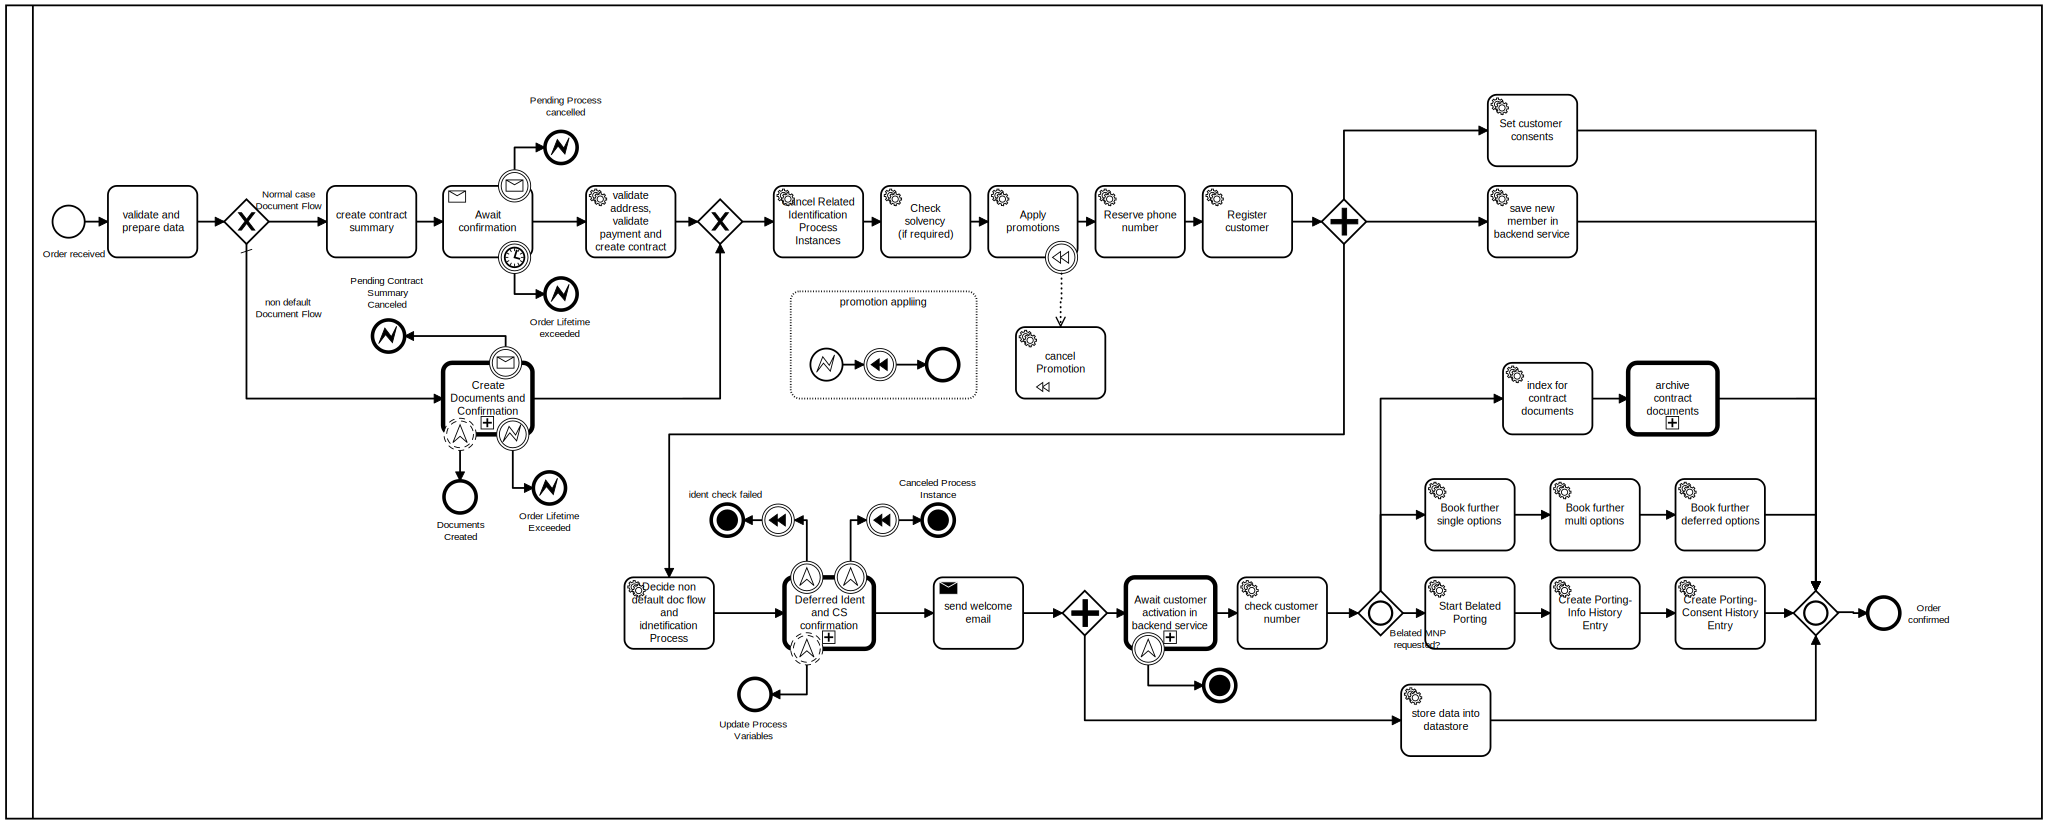
\includegraphics[width=1.7\columnwidth, angle=90 ]{graphics/process-bpmn.pdf}
	\caption{Example of a process where tasks can be merged together} 
	\label{fig:example-process} 
\end{figure}

\section{Evaluation by the Software}
\section{Comply with Naming Conventions}
%TODO
%see  https://docs.camunda.io/docs/components/best-practices/modeling/creating-readable-process-models/
%   & https://docs.camunda.io/docs/components/best-practices/modeling/naming-bpmn-elements/
\subsection{renaming tasks}
\subsection{renaming gateways}
\subsection{rename events}

\section{Extend automation boundaries}
%TODO

\section{Eliminate Manual Tasks}
%TODO

\section{Complete the process model}
%TODO

\section{No two consecutive Tasks handled by the same resource}
%TODO

\section{Inclusive Gateways over combining parallel and exclusive Gateways}
%TODO

\section{Value Added Analysis}
%TODO

\section{Evaluate Suggestions Quantitative}
%TODO



\chapter{Conclusion}
This thesis aimed to summarize best practices for creating and transforming executable BPMN models. Based on the best practices given in chapter \ref{chapter-2} and \ref{chapter-3}, the following suggestions can be implemented into a given BPMN process model:
\begin{enumerate}
	\item Comply with naming conventions
	\item Eliminate manual tasks
	\item Extend automation boundaries
	\item Complete the process model
	\item Merge consecutive tasks handled by the same resource
	\item Replace combinations of parallel and exclusive gateways with inclusive gateways
	\item Perform value added analysis and waste elimination
\end{enumerate}

The software described in chapter \ref{chapter-4} can be used to scan an \textit{.bpmn} file for violations of the mentioned best practices. The software then returns a list of BPMN elements that violate the given rule. This software is freely available as an open source project on GitHub:  \url{https://github.com/dsunaric/epms-service}. 

This thesis goes then on to demonstrate in a case study how the software can be used as an aid to implement the listed suggestions in chapter \ref{chapter-5}. 

Implementing any of the suggestions mentioned in this thesis into every process has to be evaluated. Purposefully violating best practices can have various reasons as mentioned in the introduction \ref{intro}, like compiling with legal guidelines or utilizing the benchmarking capabilities of the used \gls{wfms} to get an insight on the performance of individual activities. 

However, all suggestions for implementing efficient process models can only be seen as a guideline since there are many reasons why a more complex process model is chosen over one that complies with most or all of the guidelines. Verification if the process is in compliance with legal requirements could be one of those reasons.

While this thesis mentioned a few anti-patterns that are commonly used in executable BPMNS, there are probably many others left that could easily be automatically identified. Further research is needed to quantifiably determine the effectiveness of implementing the given suggestions with measures like the flow-node count or execution time. 

\backmatter

% Use an optional list of figures.
\listoffigures % Starred version, i.e., \listoffigures*, removes the toc entry.

% Use an optional list of tables.
\cleardoublepage % Start list of tables on the next empty right hand page.
\listoftables % Starred version, i.e., \listoftables*, removes the toc entry.

% Use an optional list of alogrithms.
\lstlistoflistings
\addcontentsline{toc}{chapter}{List of Algorithms}

% Add an index.
\printindex

% Add a glossary.
\printglossaries

% Add a bibliography.
\bibliographystyle{plain}
\bibliography{intro}

\appendix

%\chapter{Appendix}
%\section{BPMN example output}\label{app-1}
The following output shows the output of the implemented software when giving the example \ref{fig:example-process} BPMN as input.
\begin{lstlisting}[breaklines=true, language=json]
[
{
	"title": "No two consecutive Tasks should be executed by the same resource",
	"description": "Two task that are executed one after the other can be merged if they have the same enitity executing the Task. In case of User tasks this means the same usergroup is executing this task. Automated Tasks that follow each other should also always be merged to minimize flownodes.",
	"details": "The Returned Effected Elements represent a list of tasks that can be merged with its direct successor.In case that three or more tasks can be merged, this algorithm will return every Task that can be mergedwith its successor on its own. Therefore if \"task1\" , \"task2\" and \"task3\" can be merged all together, this algorithm will \"task2\" and \"task3\" as effected elements",
	"effectedElements": [
	{
		"id": "CancelRelatedWebIdent",
		"name": "Cancel Related Identification Process Instances",
		"type": "Task"
	},
	{
		"id": "ReserveMsisdn",
		"name": "Reserve phone number",
		"type": "Task"
	},
	{
		"id": "BookAutoTopups",
		"name": "Book further multi options",
		"type": "Task"
	},
	{
		"id": "ServiceTask_0p0tajd",
		"name": "Start Belated Porting",
		"type": "Task"
	},
	{
		"id": "ServiceTask_0e2r82f",
		"name": "Create Porting-Info History Entry",
		"type": "Task"
	},
	{
		"id": "BookSingleTopups",
		"name": "Book further single options",
		"type": "Task"
	}
	]
},
{
	"title": "No manual Tasks are allowed",
	"description": "Manual Tasks should not be part of an executable BPMN diagram",
	"details": "The Returned Effected Elements represent a list of manual tasks in the given diagram",
	"effectedElements": [
	{
		"id": "data_to_warehouse",
		"name": "store data into datastore",
		"type": "Task"
	}
	]
},
{
	"title": "Event based gateways instead of a parallel gateway followed by exclusive gateways",
	"description": "Event based gateways should be used instead of a parallel gateway followed by one or more exclusive gateways",
	"details": "This Rule applied whenever a parallel gateways is followed by one or more exclusive gateways. The returned Effected Elements are a list of parallel gateways that are followed by one or more exclusive gateways in the given diagram",
	"effectedElements": [
	{
		"id": "ParallelGateway_0crudor",
		"name": null,
		"type": "Gateway"
	}
	]
},
{
	"title": "Apply naming conventions",
	"description": "One aspect of naming convention is the length of labels, this rule scanns the bpmn for rlements with long labels (> 5 words)",
	"details": "The returned effected elements are all elements with a label that has more than 5 words",
	"effectedElements": [
	{
		"id": "ServiceTask_DefaultDocWorkflowPostAwaitConfirmation",
		"name": "validate address, validate payment and create contract",
		"type": "Task"
	},
	{
		"id": "DecideIdAndCsProcess",
		"name": "Decide non default doc flow and idnetification Process",
		"type": "Task"
	},
	{
		"id": "save_member_for_riskident",
		"name": "save new member in backend service",
		"type": "Task"
	}
	]
}
]
\end{lstlisting}

\end{document}